\section{Representing patterns}\label{representing-patterns}

Functional Reactive Programming (FRP) was first implemented by Conal
Elliot in Fran {[}Functional Reactive Animation; @cite{]}, based on a
formal definition of behaviour as a continuous function of time. Popular
implementations of FRP (e.g.~the Elm language) have followed which have
instead opted for discrete rather than continuous semantics. The
following introduces an approach that supports both discrete and
continuous time, developed and popularised over the past ten years in
the TidalCycles system, which is designed for creative, live exploration
of musical (and other) patterns.

In the following I will step through the process of building a
representation, taking Elliot's definition of behaviour in Fran as a
worthy starting point, and the definition of pattern in TidalCycles
(with some simplifications) as an endpoint. This is done in a practical,
literate programming style, using the Haskell programming language.
Example patterns are visualised, generated directly from the code in the
paper. We will end up with a representation that is slightly simplified
to but conceptually the same as that used in the TidalCycles programming
language.

Our starting point is the following \texttt{Behaviour} type from Fran:

\begin{Shaded}
\begin{Highlighting}[]
\KeywordTok{type} \DataTypeTok{Time} \OtherTok{=} \DataTypeTok{Double}
\KeywordTok{type} \DataTypeTok{Behaviour}\NormalTok{ a }\OtherTok{=} \DataTypeTok{Time} \OtherTok{{-}\textgreater{}}\NormalTok{ [a]}
\end{Highlighting}
\end{Shaded}

This principled start represents behaviours as functions of time, or in
other words, time-varying values. There might be more than one value
active at a particular point in time, hence the function returns a list
of values.

\subsection{Rational time}\label{rational-time}

According to Elliot, \texttt{Time} in FRP should be \emph{real},
therefore having arbitrary time precision, without building a notion of
samplerate into the representation itself. In practice, Fran uses double
precision, floating point numbers for representing time. Floating point
numbers are certainly efficient, but leave us with the problem of how to
deal with floating point errors in time calculations.

To avoid floating point headaches, here I instead use rational time as a
practical alternative. Unlike floating point numbers, this means ratios
that are common in media arts can be properly represented,
e.g.~durations of 1/3 for triplets in music, and 1/24 for frame
frequencies in video animation.

\begin{Shaded}
\begin{Highlighting}[]
\KeywordTok{type} \DataTypeTok{Time} \OtherTok{=} \DataTypeTok{Rational}
\KeywordTok{type} \DataTypeTok{Pattern}\NormalTok{ a }\OtherTok{=} \DataTypeTok{Time} \OtherTok{{-}\textgreater{}}\NormalTok{ [a]}
\end{Highlighting}
\end{Shaded}

But this raises a question -- what are these numbers a ratio \emph{of}?
The answer is metric cycles, which in music have particular meaning
depending on the musical tradition at play. For example in Western
music, metric cycles are referred to as measures or bars, and in Indian
music as the nuanced structures of Tala cycles. In TidalCycles they are
simply referred as cycles. The integer timeline (i.e., those ratios of
\texttt{1}) marks out the endings and beginnings of successive cycles.

I have also renamed the \texttt{Behaviour} type to \texttt{Pattern} in
the above. This both differentiates our type from Elliot's, and supports
later discussion relating this representation with the long history of
pattern-making.

\subsection{Timespans and events}\label{timespans-and-events}

Next, in order to support discrete events, I introduce the concept of
events with time\emph{spans} to our model. In the following, a timespan
represents the time during which a given event is active.

\begin{Shaded}
\begin{Highlighting}[]
\KeywordTok{data} \DataTypeTok{TimeSpan} \OtherTok{=} \DataTypeTok{TimeSpan}\NormalTok{ \{}\OtherTok{begin ::} \DataTypeTok{Time}\NormalTok{,}\OtherTok{ end ::} \DataTypeTok{Time}\NormalTok{\}}
\KeywordTok{data} \DataTypeTok{Event}\NormalTok{ a }\OtherTok{=} \DataTypeTok{Event}\NormalTok{ \{}\OtherTok{active ::} \DataTypeTok{TimeSpan}\NormalTok{,}\OtherTok{ value ::}\NormalTok{ a\}}
\KeywordTok{type} \DataTypeTok{Pattern}\NormalTok{ a }\OtherTok{=} \DataTypeTok{TimeSpan} \OtherTok{{-}\textgreater{}}\NormalTok{ [}\DataTypeTok{Event}\NormalTok{ a]}
\end{Highlighting}
\end{Shaded}

To support this, I have also changed the \texttt{Pattern} type to be a
function of timespans, rather than single time values. This is so the
pattern can be queried with contiguous timespans, thereby avoiding any
chance of missing events that might otherwise fall between queries of
single time values.

However, we also need to take into account that an event might well not
fit within the timespan of a given query. We often need to know which
part of an event is active within the queried timespan, particularly
whether it started before and/or continues beyond that timespan. For
this reason, I add another field to our Event datatype called
\texttt{whole}, representing the whole timespan of the event, which will
either be the same as or greater than the \texttt{active} part, but
should always include it. We still use the \texttt{active} timespan to
see when an event is active during the query, but can compare it with
the \texttt{whole} to check whether the event is a fragment of a larger
timespan.

\begin{Shaded}
\begin{Highlighting}[]
\KeywordTok{data} \DataTypeTok{Event}\NormalTok{ a }\OtherTok{=} \DataTypeTok{Event}\NormalTok{ \{}\OtherTok{whole ::} \DataTypeTok{TimeSpan}\NormalTok{,}\OtherTok{ active ::} \DataTypeTok{TimeSpan}\NormalTok{,}\OtherTok{ value ::}\NormalTok{ a\}}
\end{Highlighting}
\end{Shaded}

Now the \texttt{Pattern} type can represent discrete events, but it
would be best if it could still represent continuous values.
Fundamentally, we define a continuous value as one which does not have a
discrete beginning and end. So, we just need to make the `whole'
optional, using Haskell's standard \texttt{Maybe} type.

\begin{Shaded}
\begin{Highlighting}[]
\KeywordTok{data} \DataTypeTok{Event}\NormalTok{ a }\OtherTok{=} \DataTypeTok{Event}\NormalTok{ \{}\OtherTok{whole ::} \DataTypeTok{Maybe} \DataTypeTok{TimeSpan}\NormalTok{,}\OtherTok{ active ::} \DataTypeTok{TimeSpan}\NormalTok{,}\OtherTok{ value ::}\NormalTok{ a\}}
\end{Highlighting}
\end{Shaded}

We can now tell when an event is continuous, because its \texttt{whole}
is set to \texttt{Nothing}.

\subsection{Complete pattern
representation}\label{complete-pattern-representation}

The representation in types is now complete, with the following a basis
for representing values that support both continuous and discrete time,
within the same datatype.

\begin{Shaded}
\begin{Highlighting}[]
\KeywordTok{type} \DataTypeTok{Time} \OtherTok{=} \DataTypeTok{Rational}
\KeywordTok{data} \DataTypeTok{TimeSpan} \OtherTok{=} \DataTypeTok{TimeSpan}\NormalTok{ \{}\OtherTok{begin ::} \DataTypeTok{Time}\NormalTok{,}\OtherTok{ end ::} \DataTypeTok{Time}\NormalTok{\}}
    \KeywordTok{deriving} \DataTypeTok{Show}
\KeywordTok{data} \DataTypeTok{Event}\NormalTok{ a }\OtherTok{=} \DataTypeTok{Event}\NormalTok{ \{}\OtherTok{whole ::} \DataTypeTok{Maybe} \DataTypeTok{TimeSpan}\NormalTok{,}\OtherTok{ active ::} \DataTypeTok{TimeSpan}\NormalTok{,}\OtherTok{ value ::}\NormalTok{ a\}}
    \KeywordTok{deriving}\NormalTok{ (}\DataTypeTok{Show}\NormalTok{, }\DataTypeTok{Functor}\NormalTok{)}
\KeywordTok{data} \DataTypeTok{Pattern}\NormalTok{ a }\OtherTok{=} \DataTypeTok{Pattern}\NormalTok{ \{}\OtherTok{query ::} \DataTypeTok{TimeSpan} \OtherTok{{-}\textgreater{}}\NormalTok{ [}\DataTypeTok{Event}\NormalTok{ a]\}}
    \KeywordTok{deriving}\NormalTok{ (}\DataTypeTok{Functor}\NormalTok{)}
\end{Highlighting}
\end{Shaded}

\section{Constructing patterns}\label{constructing-patterns}

How does this work in practice? For continuous patterns, we simply
sample a value at the halfway point of the queried timespan. For
example, a sinewave:

\begin{Shaded}
\begin{Highlighting}[]
\OtherTok{sinewave ::} \DataTypeTok{Pattern} \DataTypeTok{Double}
\NormalTok{sinewave }\OtherTok{=} \DataTypeTok{Pattern} \OperatorTok{$}\NormalTok{ \textbackslash{}timespan }\OtherTok{{-}\textgreater{}}
\NormalTok{  [}\DataTypeTok{Event} \DataTypeTok{Nothing}\NormalTok{ timespan }\OperatorTok{$} \FunctionTok{sin} \OperatorTok{$}\NormalTok{ (}\FunctionTok{fromRational} \OperatorTok{$}\NormalTok{ t timespan) }\OperatorTok{*} \FunctionTok{pi} \OperatorTok{*} \DecValTok{2}\NormalTok{]}
    \KeywordTok{where}\NormalTok{ t timespan }\OtherTok{=}\NormalTok{ begin timespan }\OperatorTok{+}\NormalTok{ ((end timespan }\OperatorTok{{-}}\NormalTok{ begin timespan) }\OperatorTok{/} \DecValTok{2}\NormalTok{)}
\end{Highlighting}
\end{Shaded}

For discrete patterns however, we need to supply both the whole and
part. The following \texttt{atom} function returns a pattern that
repeats an event with the given value every cycle.

\begin{Shaded}
\begin{Highlighting}[]
\NormalTok{sam,}\OtherTok{ nextSam ::} \DataTypeTok{Rational} \OtherTok{{-}\textgreater{}} \DataTypeTok{Rational}
\NormalTok{sam t }\OtherTok{=} \FunctionTok{toRational}\NormalTok{ (}\FunctionTok{floor}\OtherTok{ t ::} \DataTypeTok{Int}\NormalTok{)}
\NormalTok{nextSam }\OtherTok{=}\NormalTok{ (}\DecValTok{1} \OperatorTok{+}\NormalTok{) }\OperatorTok{.}\NormalTok{ sam}

\OtherTok{splitSpan ::} \DataTypeTok{TimeSpan} \OtherTok{{-}\textgreater{}}\NormalTok{ [}\DataTypeTok{TimeSpan}\NormalTok{]}
\NormalTok{splitSpan (}\DataTypeTok{TimeSpan}\NormalTok{ s e) }\OperatorTok{|}\NormalTok{ sam s }\OperatorTok{==}\NormalTok{ sam e }\OperatorTok{||}\NormalTok{ n }\OperatorTok{==}\NormalTok{ e }\OtherTok{=}\NormalTok{ [}\DataTypeTok{TimeSpan}\NormalTok{ s e]}
                         \OperatorTok{|} \FunctionTok{otherwise} \OtherTok{=} \DataTypeTok{TimeSpan}\NormalTok{ s n }\OperatorTok{:}\NormalTok{ splitSpan (}\DataTypeTok{TimeSpan}\NormalTok{ n e)}
    \KeywordTok{where}\NormalTok{ n }\OtherTok{=}\NormalTok{ nextSam s}

\OtherTok{atom ::}\NormalTok{ a }\OtherTok{{-}\textgreater{}} \DataTypeTok{Pattern}\NormalTok{ a}
\NormalTok{atom value }\OtherTok{=} \DataTypeTok{Pattern} \OperatorTok{$} \FunctionTok{map}\NormalTok{ (\textbackslash{}timespan }\OtherTok{{-}\textgreater{}}
                              \DataTypeTok{Event}\NormalTok{ (}\DataTypeTok{Just} \OperatorTok{$} \DataTypeTok{TimeSpan}\NormalTok{ (sam }\OperatorTok{$}\NormalTok{ begin timespan)}
\NormalTok{                                                     (nextSam }\OperatorTok{$}\NormalTok{ begin timespan)}
\NormalTok{                                    )}
\NormalTok{                                    timespan}
\NormalTok{                                    value}
\NormalTok{                           ) }\OperatorTok{.}\NormalTok{ splitSpan}
\end{Highlighting}
\end{Shaded}

\section{Composing patterns}\label{composing-patterns}

We can compose a list of patterns into a new one, simply by passing
queries on to each pattern. This assumes that we want the patterns to
run concurrently:

\begin{Shaded}
\begin{Highlighting}[]
\OtherTok{stack ::}\NormalTok{ [}\DataTypeTok{Pattern}\NormalTok{ a] }\OtherTok{{-}\textgreater{}} \DataTypeTok{Pattern}\NormalTok{ a}
\NormalTok{stack pats }\OtherTok{=} \DataTypeTok{Pattern} \OperatorTok{$}\NormalTok{ \textbackslash{}timespan }\OtherTok{{-}\textgreater{}} \FunctionTok{concatMap}\NormalTok{ (}\OtherTok{\textasciigrave{}query\textasciigrave{}}\NormalTok{ timespan) pats}
\end{Highlighting}
\end{Shaded}

\begin{Shaded}
\begin{Highlighting}[]
\NormalTok{fig1 }\OtherTok{=}\NormalTok{ stack [atom }\StringTok{"pink"}\NormalTok{, atom }\StringTok{"purple"}\NormalTok{]}
\end{Highlighting}
\end{Shaded}

\includegraphics{../figures/fig1.pdf}\\

The above visualises twelve cycles of the pattern over time, from left
to right. Slightly more complicated is combining patterns in sequence,
over time. Patterns have infinite length, so we are not able to simply
concatenate them. Instead, we can `interlace' their cycles.

\begin{Shaded}
\begin{Highlighting}[]
\OtherTok{splitQueries ::} \DataTypeTok{Pattern}\NormalTok{ a }\OtherTok{{-}\textgreater{}} \DataTypeTok{Pattern}\NormalTok{ a}
\NormalTok{splitQueries pat }\OtherTok{=}  \DataTypeTok{Pattern} \OperatorTok{$} \FunctionTok{concatMap}\NormalTok{ (query pat) }\OperatorTok{.}\NormalTok{ splitSpan}

\OtherTok{interlace ::}\NormalTok{ [}\DataTypeTok{Pattern}\NormalTok{ a] }\OtherTok{{-}\textgreater{}} \DataTypeTok{Pattern}\NormalTok{ a}
\NormalTok{interlace pats }\OtherTok{=}\NormalTok{ splitQueries }\OperatorTok{$} \DataTypeTok{Pattern}\NormalTok{ f}
  \KeywordTok{where}\NormalTok{ f timespan }\OtherTok{=}\NormalTok{ query (\_late offset pat) timespan}
              \KeywordTok{where}\NormalTok{ n }\OtherTok{=} \FunctionTok{toRational} \OperatorTok{$} \FunctionTok{length}\NormalTok{ pats}
\NormalTok{                    cyc }\OtherTok{=}\NormalTok{ sam }\OperatorTok{$}\NormalTok{ begin timespan}
\NormalTok{                    pat }\OtherTok{=}\NormalTok{ pats }\OperatorTok{!!} \FunctionTok{floor}\NormalTok{ (cyc }\OtherTok{\textasciigrave{}mod\textquotesingle{}\textasciigrave{}}\NormalTok{ (}\OtherTok{n ::} \DataTypeTok{Rational}\NormalTok{))}
\NormalTok{                    offset }\OtherTok{=}\NormalTok{ cyc }\OperatorTok{{-}}\NormalTok{ sam (begin timespan }\OperatorTok{/}\NormalTok{ n)}
\end{Highlighting}
\end{Shaded}

Let's look at a visualisation of the first six cycles of a pattern
composed using both \texttt{interlace} and \texttt{stack}. In the
following time is from left to right, with the vertical axis used to
show simultaneously occuring events.

\begin{Shaded}
\begin{Highlighting}[]
\NormalTok{fig2 }\OtherTok{=}\NormalTok{ interlace [atom }\StringTok{"pink"}\NormalTok{, atom }\StringTok{"purple"}\NormalTok{]}
\end{Highlighting}
\end{Shaded}

\includegraphics{../figures/fig2.pdf}\\

We can now combine stacks and interlacements:

\begin{Shaded}
\begin{Highlighting}[]
\NormalTok{fig3 }\OtherTok{=}\NormalTok{ stack [atom }\StringTok{"red"}\NormalTok{, interlace [atom }\StringTok{"pink"}\NormalTok{, atom }\StringTok{"purple"}\NormalTok{]]}
\end{Highlighting}
\end{Shaded}

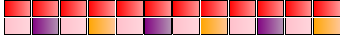
\includegraphics{../figures/fig3.pdf}\\

\section{Manipulating time}\label{manipulating-time}

A good thing about pure FRP is that it is possible to manipulate time
simply by making a new pattern function that simply adjusts the time
query that is passed to an existing pattern function. However, because
our representation has timespans in two places -- in the query and the
events that result -- we must be careful to adjust both. We therefore
require two functions for every time manipulation; one to adjust the
query, and another to adjust the result, so that the event timespan are
still active within the queried timespan. To facilitate this, I first
define some utility functions for working with query and event time:

\begin{Shaded}
\begin{Highlighting}[]
\OtherTok{withSpanTime ::}\NormalTok{ (}\DataTypeTok{Time} \OtherTok{{-}\textgreater{}} \DataTypeTok{Time}\NormalTok{) }\OtherTok{{-}\textgreater{}} \DataTypeTok{TimeSpan} \OtherTok{{-}\textgreater{}} \DataTypeTok{TimeSpan}
\NormalTok{withSpanTime timef (}\DataTypeTok{TimeSpan}\NormalTok{ b e) }\OtherTok{=} \DataTypeTok{TimeSpan}\NormalTok{ (timef b) (timef e)}

\OtherTok{withQueryTime ::}\NormalTok{ (}\DataTypeTok{Time} \OtherTok{{-}\textgreater{}} \DataTypeTok{Time}\NormalTok{) }\OtherTok{{-}\textgreater{}} \DataTypeTok{Pattern}\NormalTok{ a }\OtherTok{{-}\textgreater{}} \DataTypeTok{Pattern}\NormalTok{ a}
\NormalTok{withQueryTime timef (}\DataTypeTok{Pattern}\NormalTok{ q) }\OtherTok{=} \DataTypeTok{Pattern} \OperatorTok{$}\NormalTok{ q }\OperatorTok{.}\NormalTok{ withSpanTime timef}

\OtherTok{withEventTime ::}\NormalTok{ (}\DataTypeTok{Time} \OtherTok{{-}\textgreater{}} \DataTypeTok{Time}\NormalTok{) }\OtherTok{{-}\textgreater{}} \DataTypeTok{Pattern}\NormalTok{ a }\OtherTok{{-}\textgreater{}} \DataTypeTok{Pattern}\NormalTok{ a}
\NormalTok{withEventTime f }\OtherTok{=}\NormalTok{ withEvent }\OperatorTok{$}\NormalTok{ \textbackslash{}e }\OtherTok{{-}\textgreater{}}\NormalTok{ e \{active }\OtherTok{=}\NormalTok{ withSpanTime f }\OperatorTok{$}\NormalTok{ active e,}
\NormalTok{                                       whole }\OtherTok{=}\NormalTok{ withSpanTime f }\OperatorTok{\textless{}$\textgreater{}}\NormalTok{ whole e}
\NormalTok{                                      \}}
    \KeywordTok{where}\NormalTok{ withEvent ef (}\DataTypeTok{Pattern}\NormalTok{ q) }\OtherTok{=} \DataTypeTok{Pattern} \OperatorTok{$} \FunctionTok{map}\NormalTok{ ef }\OperatorTok{\textless{}$\textgreater{}}\NormalTok{ q}

\OtherTok{withTime ::}\NormalTok{ (}\DataTypeTok{Time} \OtherTok{{-}\textgreater{}} \DataTypeTok{Time}\NormalTok{) }\OtherTok{{-}\textgreater{}}\NormalTok{ (}\DataTypeTok{Time} \OtherTok{{-}\textgreater{}} \DataTypeTok{Time}\NormalTok{) }\OtherTok{{-}\textgreater{}} \DataTypeTok{Pattern}\NormalTok{ a }\OtherTok{{-}\textgreater{}} \DataTypeTok{Pattern}\NormalTok{ a}
\NormalTok{withTime fa fb pat }\OtherTok{=}\NormalTok{ withEventTime fa }\OperatorTok{$}\NormalTok{ withQueryTime fb pat}
\end{Highlighting}
\end{Shaded}

It is then straightforward to define functions for making patterned
events faster/slower, or early/late. For example to make a pattern
`faster', query time is divided and event time is multiplied by a given
factor. This queries a wider window, and `squashes' the results back
into the requested timespan.

\begin{Shaded}
\begin{Highlighting}[]
\NormalTok{\_fast, \_slow, \_late,}\OtherTok{ \_early ::} \DataTypeTok{Time} \OtherTok{{-}\textgreater{}} \DataTypeTok{Pattern}\NormalTok{ a }\OtherTok{{-}\textgreater{}} \DataTypeTok{Pattern}\NormalTok{ a}
\NormalTok{\_fast t  }\OtherTok{=}\NormalTok{ withEventTime (}\OperatorTok{/}\NormalTok{ t) }\OperatorTok{.}\NormalTok{ withQueryTime (}\OperatorTok{*}\NormalTok{ t)}
\NormalTok{\_slow t  }\OtherTok{=}\NormalTok{ withEventTime (}\OperatorTok{*}\NormalTok{ t) }\OperatorTok{.}\NormalTok{ withQueryTime (}\OperatorTok{/}\NormalTok{ t)}
\NormalTok{\_early t }\OtherTok{=}\NormalTok{ withEventTime (}\FunctionTok{subtract}\NormalTok{ t) }\OperatorTok{.}\NormalTok{ withQueryTime (}\OperatorTok{+}\NormalTok{ t)}
\NormalTok{\_late t  }\OtherTok{=}\NormalTok{ withEventTime (}\OperatorTok{+}\NormalTok{ t) }\OperatorTok{.}\NormalTok{ withQueryTime (}\FunctionTok{subtract}\NormalTok{ t)}
\end{Highlighting}
\end{Shaded}

We can apply visualisation in understanding how events can become broken
up. If \texttt{interlace} works cycle-by-cycle, what happens if an event
lasts longer than a cycle?

\begin{Shaded}
\begin{Highlighting}[]
\NormalTok{fig4 }\OtherTok{=}\NormalTok{ interlace [atom }\StringTok{"red"}\NormalTok{, \_slow }\DecValTok{3} \OperatorTok{$}\NormalTok{ atom }\StringTok{"yellow"}\NormalTok{]}
\end{Highlighting}
\end{Shaded}

\includegraphics{../figures/fig4.pdf}\\

The dashed lines indicate where wholes begin before, or end after, the
active event timespans. From the above we can see that the three cycles
of each yellow event has been broken into parts of one cycle each, and
interlaced with the single-cycle red events.

\subsection{Combining patterns with monadic
binds}\label{combining-patterns-with-monadic-binds}

On these foundations, a domain specific language can be built. The above
functions are prefixed by \texttt{\_}, because they are considered
internal functions and not part of the end-user interface. The reason
for this is that TidalCycles follows the principle that
\emph{everything} is a pattern. Accordingly, we require functions with
the following time signature:

\begin{Shaded}
\begin{Highlighting}[]
\NormalTok{fast, slow, late,}\OtherTok{ early ::} \DataTypeTok{Pattern} \DataTypeTok{Time} \OtherTok{{-}\textgreater{}} \DataTypeTok{Pattern}\NormalTok{ a }\OtherTok{{-}\textgreater{}} \DataTypeTok{Pattern}\NormalTok{ a}
\end{Highlighting}
\end{Shaded}

How do we implement these functions? We somehow need a way to combine
patterns of time with the patterns that are having their time structures
manipulated. This is where Haskell's monadic bind
(\texttt{\textgreater{}\textgreater{}=}) comes into view, which does
what we want - it lifts functional arguments into contexts such as
patterns. This clarifies our problem as one of how to define patterns as
an instance of Haskell's standard Monad typeclass. In particular, we
need to define the bind operator \texttt{\textgreater{}\textgreater{}=}
for patterns, with the type signature
\texttt{Pattern\ a\ -\textgreater{}\ (a\ -\textgreater{}\ Pattern\ b)\ -\textgreater{}\ Pattern\ b}.
So, what should this bind do?

Certainly, our bind will need to create a new pattern, which as we saw
above, will be a function from timespans to events. This function will
need to be composed of other pattern functions, in particular the
`outer' pattern given as the first argument, and `inner' pattern
resulting from the second argument. The biggest question here is
deciding how to deal with the timespans of events when composing pairs
of patterns together. The two active timespans are straightforwardly
combined, as the intersection. There is however ambiguity in how the two
`whole' timespans should be combined.

\href{}{//}: \textless\textgreater{} The events returned from those
inner pattern queries are then collated and returned, with one caveat --
there is ambiguity about what the resulting event's `whole' timespan
should be. It could from from the `outer' or `inner' pattern, or be the
intersection of the two.

This ambiguity comes down to where the pattern \emph{structure} should
come from - should we preserve the structure of the outer pattern, the
inner pattern, or a combination of the two? In the case of the above
\texttt{fast} function and its \texttt{slow}, \texttt{late} and
\texttt{early} friends, we can say that we will always want to preserve
the structure of the inner patterns - the patterns of values which come
second in the function arguments. This is because we only want to
transform a value pattern using a time pattern, but not otherwise change
the value pattern's structure. (We will see examples of functions that
do change the structure of events later.)

The following shows how inner, outer and `mix' binds can be implemented.

\begin{Shaded}
\begin{Highlighting}[]
\OtherTok{bindWith ::}\NormalTok{ (}\DataTypeTok{Maybe} \DataTypeTok{TimeSpan} \OtherTok{{-}\textgreater{}} \DataTypeTok{Maybe} \DataTypeTok{TimeSpan} \OtherTok{{-}\textgreater{}} \DataTypeTok{Maybe} \DataTypeTok{TimeSpan}\NormalTok{) }\OtherTok{{-}\textgreater{}}
                \DataTypeTok{Pattern}\NormalTok{ a }\OtherTok{{-}\textgreater{}}\NormalTok{ (a }\OtherTok{{-}\textgreater{}} \DataTypeTok{Pattern}\NormalTok{ b) }\OtherTok{{-}\textgreater{}} \DataTypeTok{Pattern}\NormalTok{ b}
\NormalTok{bindWith chooseWhole bv f }\OtherTok{=} \DataTypeTok{Pattern} \OperatorTok{$} \FunctionTok{concatMap}\NormalTok{ match }\OperatorTok{.}\NormalTok{ query bv}
  \KeywordTok{where}\NormalTok{ match e }\OtherTok{=} \FunctionTok{map}\NormalTok{ (withWhole e) }\OperatorTok{$}\NormalTok{ query (f }\OperatorTok{$}\NormalTok{ value e) }\OperatorTok{$}\NormalTok{ active e}
\NormalTok{        withWhole e e\textquotesingle{} }\OtherTok{=}\NormalTok{ e\textquotesingle{} \{whole }\OtherTok{=}\NormalTok{ chooseWhole (whole e) (whole e\textquotesingle{})\}}

\OtherTok{innerBind ::} \DataTypeTok{Pattern}\NormalTok{ a }\OtherTok{{-}\textgreater{}}\NormalTok{ (a }\OtherTok{{-}\textgreater{}} \DataTypeTok{Pattern}\NormalTok{ b) }\OtherTok{{-}\textgreater{}} \DataTypeTok{Pattern}\NormalTok{ b}
\NormalTok{innerBind }\OtherTok{=}\NormalTok{ bindWith (}\FunctionTok{flip} \FunctionTok{const}\NormalTok{)}

\OtherTok{outerBind ::} \DataTypeTok{Pattern}\NormalTok{ a }\OtherTok{{-}\textgreater{}}\NormalTok{ (a }\OtherTok{{-}\textgreater{}} \DataTypeTok{Pattern}\NormalTok{ b) }\OtherTok{{-}\textgreater{}} \DataTypeTok{Pattern}\NormalTok{ b}
\NormalTok{outerBind }\OtherTok{=}\NormalTok{ bindWith }\FunctionTok{const}

\OtherTok{mixBind ::} \DataTypeTok{Pattern}\NormalTok{ a }\OtherTok{{-}\textgreater{}}\NormalTok{ (a }\OtherTok{{-}\textgreater{}} \DataTypeTok{Pattern}\NormalTok{ b) }\OtherTok{{-}\textgreater{}} \DataTypeTok{Pattern}\NormalTok{ b}
\NormalTok{mixBind }\OtherTok{=}\NormalTok{ bindWith (liftA2 intersect)}
\end{Highlighting}
\end{Shaded}

In \texttt{mixBind}, the intersection of the event wholes is taken,
therefore combining the time structures of the two patterns in what we
term a `mix' bind.

Alternatively, \texttt{innerBind} uses the time structure of `whole'
timespans from the inner pattern, and \texttt{outerBind} from the outer
pattern. The default bind in the \texttt{Monad} instance is set as a
\texttt{mixBind}. I also define an \texttt{Applicative} instance based
on this bind.

\begin{Shaded}
\begin{Highlighting}[]
\KeywordTok{instance} \DataTypeTok{Monad} \DataTypeTok{Pattern} \KeywordTok{where}
\NormalTok{  (}\OperatorTok{\textgreater{}\textgreater{}=}\NormalTok{) }\OtherTok{=}\NormalTok{ mixBind}

\KeywordTok{instance} \DataTypeTok{Applicative} \DataTypeTok{Pattern} \KeywordTok{where}
  \FunctionTok{pure} \OtherTok{=}\NormalTok{ atom}
\NormalTok{  pf }\OperatorTok{\textless{}*\textgreater{}}\NormalTok{ px }\OtherTok{=}\NormalTok{ pf }\OperatorTok{\textgreater{}\textgreater{}=}\NormalTok{ (}\OperatorTok{\textless{}$\textgreater{}}\NormalTok{ px)}
\end{Highlighting}
\end{Shaded}

Using this, we can make a function \texttt{patternify\_x} that lifts a
function's first argument into a pattern, using \texttt{innerBind} to
preserve the structure of the second argument. This can then be used to
define our \texttt{fast}, \texttt{slow}, \texttt{late} and
\texttt{early} functions.

\begin{Shaded}
\begin{Highlighting}[]
\OtherTok{patternify\_x ::}\NormalTok{ (a }\OtherTok{{-}\textgreater{}} \DataTypeTok{Pattern}\NormalTok{ b }\OtherTok{{-}\textgreater{}} \DataTypeTok{Pattern}\NormalTok{ c) }\OtherTok{{-}\textgreater{}}
\NormalTok{  (}\DataTypeTok{Pattern}\NormalTok{ a }\OtherTok{{-}\textgreater{}} \DataTypeTok{Pattern}\NormalTok{ b }\OtherTok{{-}\textgreater{}} \DataTypeTok{Pattern}\NormalTok{ c)}
\NormalTok{patternify\_x f ba bb }\OtherTok{=}\NormalTok{ ba }\OtherTok{\textasciigrave{}innerBind\textasciigrave{}}\NormalTok{ \textbackslash{}a }\OtherTok{{-}\textgreater{}}\NormalTok{ f a bb}

\NormalTok{fast, slow, late,}\OtherTok{ early ::} \DataTypeTok{Pattern} \DataTypeTok{Time} \OtherTok{{-}\textgreater{}} \DataTypeTok{Pattern}\NormalTok{ a }\OtherTok{{-}\textgreater{}} \DataTypeTok{Pattern}\NormalTok{ a}
\NormalTok{fast }\OtherTok{=}\NormalTok{ patternify\_x \_fast}
\NormalTok{slow }\OtherTok{=}\NormalTok{ patternify\_x \_slow}
\NormalTok{late }\OtherTok{=}\NormalTok{ patternify\_x \_late}
\NormalTok{early }\OtherTok{=}\NormalTok{ patternify\_x \_early}
\end{Highlighting}
\end{Shaded}

\begin{Shaded}
\begin{Highlighting}[]
\NormalTok{fig5 }\OtherTok{=}\NormalTok{ stack [fast (atom }\DecValTok{2}\NormalTok{) p,}
\NormalTok{              slow (atom }\DecValTok{2}\NormalTok{) p}
\NormalTok{             ]}
    \KeywordTok{where}\NormalTok{ p }\OtherTok{=}\NormalTok{ interlace [atom }\StringTok{"red"}\NormalTok{, atom }\StringTok{"purple"}\NormalTok{]}
\end{Highlighting}
\end{Shaded}

\includegraphics{../figures/fig5.pdf}\\

From the above we can see that for the second pattern in the stack
transformed with \texttt{slow}, because the \texttt{atom\ 2} repeats
every cycle, the resulting events get split at cycle boundaries. However
they keep their whole timespans with a duration of two cycles, and so
the overall time structure is maintained. In the visualisations, events
are filled with a gradient relative to the whole timespans, to make this
a little clearer.

\section{Masking and restructuring
patterns}\label{masking-and-restructuring-patterns}

So far we have manipulated time, but not structure.

\begin{Shaded}
\begin{Highlighting}[]
\OtherTok{silence ::} \DataTypeTok{Pattern}\NormalTok{ a}
\NormalTok{silence }\OtherTok{=} \DataTypeTok{Pattern} \OperatorTok{$} \FunctionTok{const}\NormalTok{ []}

\OtherTok{\_ifpat ::} \DataTypeTok{Bool} \OtherTok{{-}\textgreater{}} \DataTypeTok{Pattern}\NormalTok{ a }\OtherTok{{-}\textgreater{}} \DataTypeTok{Pattern}\NormalTok{ a}
\NormalTok{\_ifpat }\DataTypeTok{True}\NormalTok{ p }\OtherTok{=}\NormalTok{ p}
\NormalTok{\_ifpat }\DataTypeTok{False}\NormalTok{ \_ }\OtherTok{=}\NormalTok{ silence}

\OtherTok{mask ::} \DataTypeTok{Pattern} \DataTypeTok{Bool} \OtherTok{{-}\textgreater{}} \DataTypeTok{Pattern}\NormalTok{ a }\OtherTok{{-}\textgreater{}} \DataTypeTok{Pattern}\NormalTok{ a}
\NormalTok{mask bp p }\OtherTok{=}\NormalTok{ bp }\OtherTok{\textasciigrave{}outerBind\textasciigrave{}}\NormalTok{ \textbackslash{}b }\OtherTok{{-}\textgreater{}}\NormalTok{ \_ifpat b p}

\OtherTok{struct ::} \DataTypeTok{Pattern} \DataTypeTok{Bool} \OtherTok{{-}\textgreater{}} \DataTypeTok{Pattern}\NormalTok{ a }\OtherTok{{-}\textgreater{}} \DataTypeTok{Pattern}\NormalTok{ a}
\NormalTok{struct bp p }\OtherTok{=}\NormalTok{ bp }\OtherTok{\textasciigrave{}innerBind\textasciigrave{}}\NormalTok{ \textbackslash{}b }\OtherTok{{-}\textgreater{}}\NormalTok{ \_ifpat b p}
\end{Highlighting}
\end{Shaded}

\appendix

\section{Preamble and supporting
functions}\label{preamble-and-supporting-functions}

\begin{Shaded}
\begin{Highlighting}[]
\KeywordTok{module} \DataTypeTok{Pattern} \KeywordTok{where}

\KeywordTok{import} \DataTypeTok{Control.Applicative}
\KeywordTok{import} \DataTypeTok{Data.Fixed}

\OtherTok{intersect ::} \DataTypeTok{TimeSpan} \OtherTok{{-}\textgreater{}} \DataTypeTok{TimeSpan} \OtherTok{{-}\textgreater{}} \DataTypeTok{TimeSpan}
\NormalTok{intersect (}\DataTypeTok{TimeSpan}\NormalTok{ b e) (}\DataTypeTok{TimeSpan}\NormalTok{ b\textquotesingle{} e\textquotesingle{}) }\OtherTok{=} \DataTypeTok{TimeSpan}\NormalTok{ (}\FunctionTok{max}\NormalTok{ b b\textquotesingle{}) (}\FunctionTok{min}\NormalTok{ e e\textquotesingle{})}
\end{Highlighting}
\end{Shaded}
